\documentclass[tikz,border=9pt]{standalone}
\usepackage[utf8]{inputenc}
\usepackage[OT4,plmath]{polski}
\usepackage{amsmath}
\begin{document}
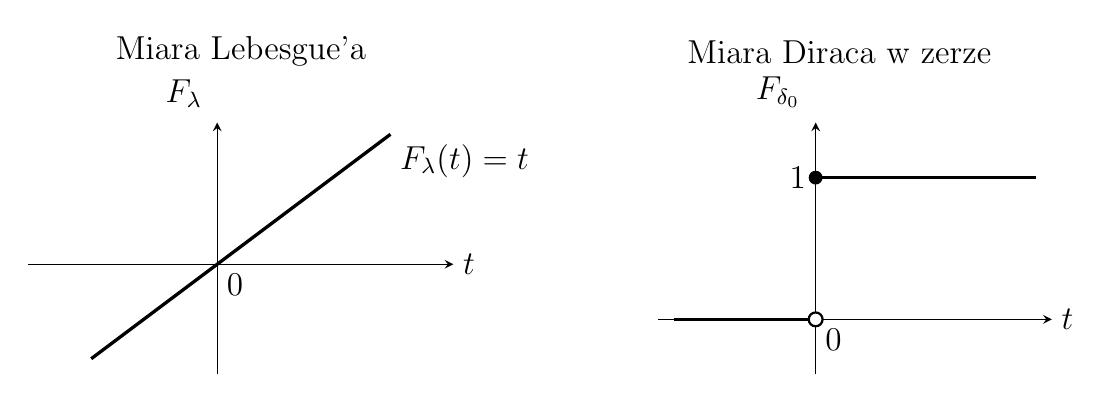
\begin{tikzpicture}[font=\large,>=stealth]
  \begin{scope}
    \node at (2.7,4.1) {Miara Lebesgue'a};
    \draw[->] (0,1.4)--(5.4,1.4) node[right] {$t$};
    \draw[->] (2.4,0)--(2.4,3.2) node[above left=2pt] {$F_\lambda$};
    \draw[very thick] (0.8,0.2)--(4.6,3.05);
    \node[below right] at (2.4,1.4) {$0$};
    \node[below right] at (4.6,3.05) {$F_\lambda(t)=t$};
  \end{scope}
  \begin{scope}[xshift=8cm]
    \node at (2.3,4.1) {Miara Diraca w zerze};
    \draw[->] (0,0.7)--(5,0.7) node[right] {$t$};
    \draw[->] (2,0)--(2,3.2) node[above left=2pt] {$F_{\delta_0}$};
    \draw[very thick] (0.2,0.7)--(2,0.7);
    \draw[very thick] (2,2.5)--(4.8,2.5);
    \filldraw[fill=white,thick] (2,0.7) circle (2.5pt);
    \fill (2,2.5) circle (2.5pt);
    \node[below right] at (2,0.7) {$0$};
    \node[left] at (2,2.5) {$1$};
  \end{scope}
\end{tikzpicture}
\end{document}
